% CVPR 2027 Paper Template; see https://github.com/cvpr-org/author-kit

\documentclass[10pt,twocolumn,letterpaper]{article}

%%%%%%%%% PAPER TYPE  - PLEASE UPDATE FOR FINAL VERSION
% \usepackage{cvpr}              % To produce the CAMERA-READY version
\usepackage[review]{cvpr}      % To produce the REVIEW version
% \usepackage[pagenumbers]{cvpr} % To force page numbers, e.g. for an arXiv version

% Import additional packages in the preamble file, before hyperref
%% This file contains a number of tweaks that are typically applied to the main document.
%% They are not enabled by default, but can be enabled by uncommenting the relevant lines.

%%
%% Inline annotations; for predefined colors, refer to "dvipsnames" in the xcolor package:
%% https://tinyurl.com/overleaf-colors
%%
\newcommand{\red}[1]{{\color{red}#1}}
\newcommand{\todo}[1]{{\color{red}#1}}
\newcommand{\TODO}[1]{\textbf{\color{red}[TODO: #1]}}
%%
%% disable for camera ready / submission by uncommenting these lines  
%%
% \renewcommand{\TODO}[1]{}
% \renewcommand{\todo}[1]{#1}

%%
%% work harder in optimizing text layout. Typically shrinks text by 1/6 of page, enable
%% it at the very end of the writing process, when you are just above the page limit
%%
% \usepackage{microtype}

%%
%% fine-tune paragraph spacing
%%
% \renewcommand{\paragraph}[1]{\vspace{.5em}\noindent\textbf{#1.}}

%%
%% globally adjusts space between figure and caption
%%
% \setlength{\abovecaptionskip}{.5em}


%%
%% Allows "the use of \paper to refer to the project name"
%% with automatic management of space at the end of the word
%%
% \usepackage{xspace}
% \newcommand{\paper}{ProjectName\xspace}

%%
%% Commonly used math definitions
%%
% \DeclareMathOperator*{\argmin}{arg\,min}
% \DeclareMathOperator*{\argmax}{arg\,max}

%%
%% Tigthen underline
%%
% \usepackage{soul}
% \setuldepth{foobar}

% It is strongly recommended to use hyperref, especially for the review version.
% hyperref with option pagebackref eases the reviewers' job.
% Please disable hyperref *only* if you encounter grave issues, 
% e.g. with the file validation for the camera-ready version.
%
% If you comment hyperref and then uncomment it, you should delete *.aux before re-running LaTeX.
% (Or just hit 'q' on the first LaTeX run, let it finish, and you should be clear).
\definecolor{cvprblue}{rgb}{0.21,0.49,0.74}
\usepackage[pagebackref,breaklinks,colorlinks,allcolors=cvprblue]{hyperref}

\def\confName{CVPR}
\def\confYear{2027}

%%%%%%%%% TITLE - PLEASE UPDATE
% LAVi stands for Low-Altitude Visual.
\title{LAVi: Low-Altitude Visual World Modeling with Geometric Supervision}

%%%%%%%%% AUTHORS - PLEASE UPDATE
\author{First Author\\
Institution1\\
Institution1 address\\
{\tt\small firstauthor@i1.org}
% For a paper whose authors are all at the same institution,
% omit the following lines up until the closing ``}''.
% Additional authors and addresses can be added with ``\and'',
% just like the second author.
% To save space, use either the email address or home page, not both
\and
Second Author\\
Institution2\\
First line of institution2 address\\
{\tt\small secondauthor@i2.org}
}

% Keep the teaser inside the full-width title block, above the abstract.
\makeatletter
\g@addto@macro\@maketitle{%
    \noindent\begin{minipage}{\textwidth}
        \centering
        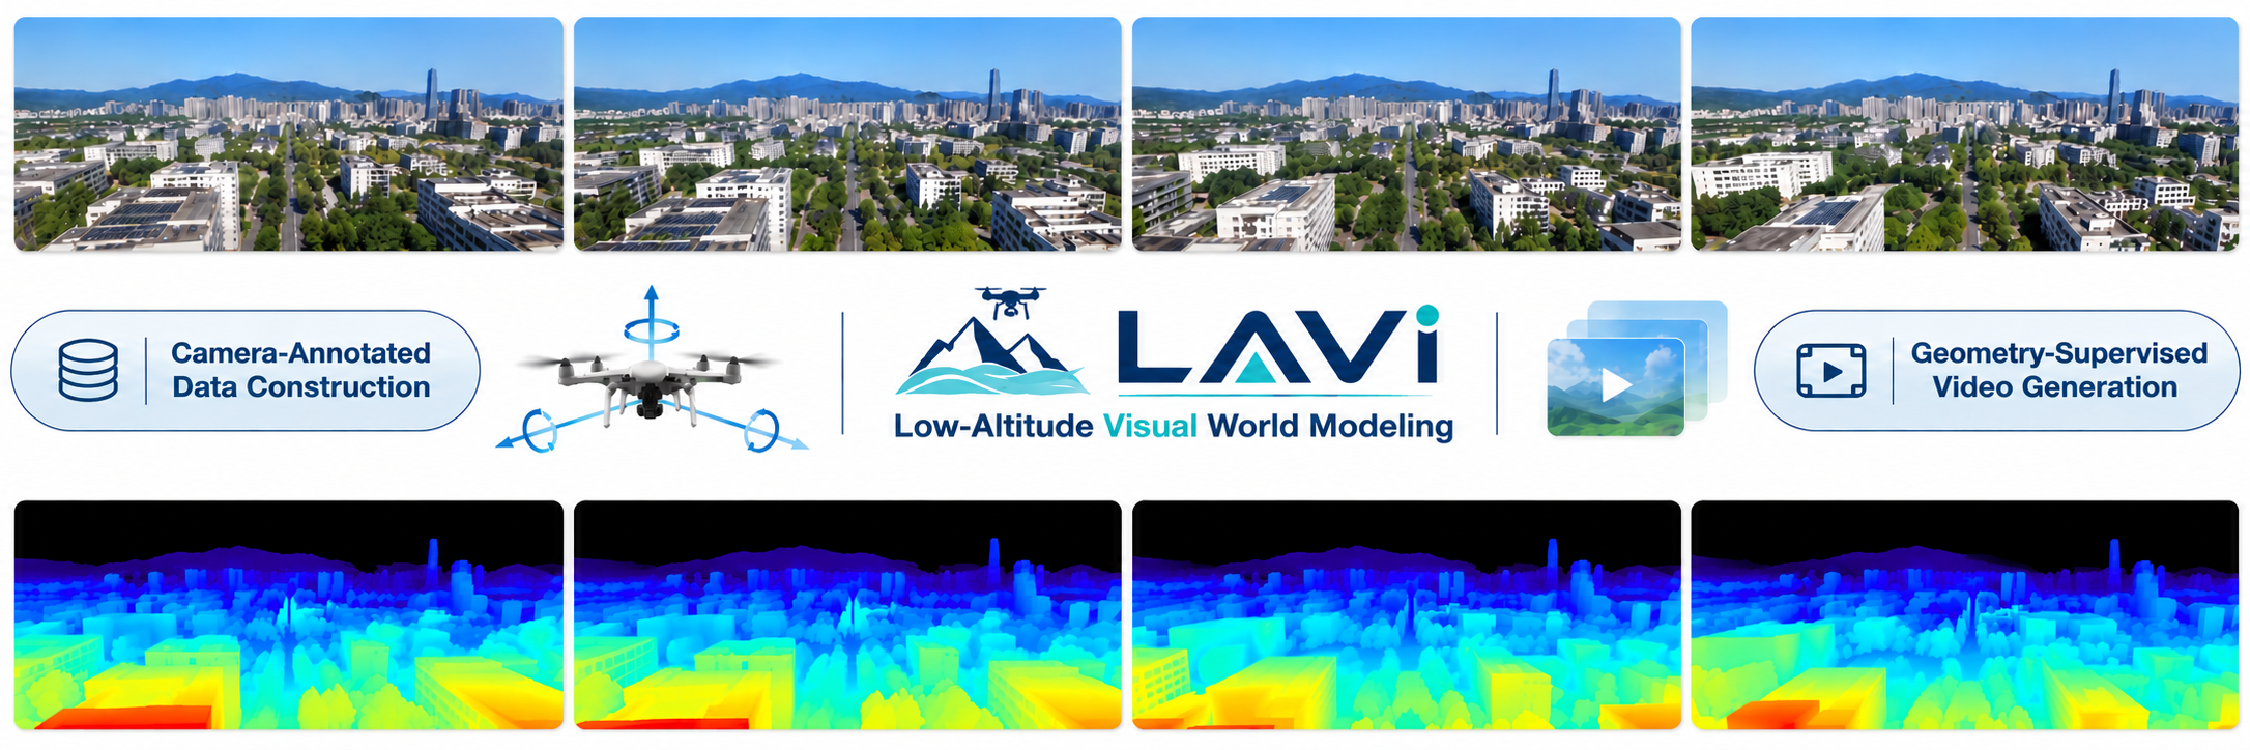
\includegraphics[width=\linewidth]{figures/LAVi.pdf}
        \captionof{figure}{\textbf{LAVi for low-altitude visual world modeling.} Given an initial image, text, and a planned camera trajectory, LAVi jointly predicts RGB observations and depth. Camera-annotated data and geometric supervision support controllable UAV simulation and navigation.}
        \label{fig:teaser}
    \end{minipage}\par
    \vspace{12pt}%
}
\makeatother

\begin{document}
\maketitle
% Each section is maintained in its own file.
% Official author-kit examples are archived in template_examples/sec/.
% !TeX root = ../main.tex
\begin{abstract}
Visual world models offer a foundation for low-altitude unmanned aerial vehicle (UAV) simulation and navigation by predicting future observations along planned flight trajectories.
However, missing camera annotations and inconsistent coordinate conventions and translation scales limit the reliability of supervision assembled from heterogeneous video sources.
For camera-conditioned models trained only on RGB targets, scene structure remains implicit in the prediction objective, without direct depth supervision to constrain viewpoint-dependent geometry.
We propose \textbf{LAVi}, a unified framework for \textbf{L}ow-\textbf{A}ltitude \textbf{Vi}sual world modeling that couples camera-annotated data construction with geometry-supervised video generation.
We assemble 600,000 clips spanning simulation, public videos, and real UAV flights, including 200,000 simulated clips whose ground-truth trajectories guide metric-scale calibration and pose-estimator selection for camera annotation across sources.
A shared transformer with modality-specific prediction branches jointly generates RGB frames and depth maps, using metric-depth supervision to constrain scene geometry and scale.
We directly adapt the bidirectionally trained model to few-step causal generation by combining future-frame alignment under reference histories with feature-space distribution matching of self-generated rollouts.
Experiments show that our data construction strategy and geometry-supervised generation method together enable LAVi to achieve the best camera-control accuracy and visual fidelity among the evaluated world models.
\end{abstract}

% !TeX root = ../main.tex
% Revised 2026-10-18: expanded primary-source citation traceback; implementation/results TODOs are intentional.
\section{Introduction}
\label{sec:intro}


Visual world models aim to predict how an environment evolves by generating future observations conditioned on current observations and actions~\cite{ha2018worldmodels,yang2024learninginteractiverealworldsimulators,hu2023gaia1generativeworldmodel}.
%
Building on advances in video generation~\cite{ho2022videodiffusionmodels,blattmann2023stablevideodiffusionscaling,yang2025cogvideoxtexttovideodiffusionmodels,kong2025hunyuanvideosystematicframeworklarge,wan2025wanopenadvancedlargescale}, recent models have enabled increasingly realistic and controllable visual rollouts driven by action inputs~\cite{bruce2024geniegenerativeinteractiveenvironments,valevski2025diffusionmodelsrealtimegame,he2026matrixgame20opensourcerealtime,zhang2026worldplay2extendingrealtimeinteractive,zhou2026astronexworld10realtimeinteractive} and camera trajectories~\cite{he2025cameractrlenablingcameracontrol,wang2024motionctrlunifiedflexiblemotion,xu2024camcocameracontrollable3dconsistentimagetovideo,zhang2026unifiedcamerapositionalencoding,huang2026solarwmopendatascalable,zhu2026sanawmefficientminutescaleworld}.
%
By predicting future observations under different actions or camera trajectories, these models provide a foundation for simulation, planning, and decision-making~\cite{yang2024learninginteractiverealworldsimulators,alonso2024diffusionworldmodelingvisual,gao2026dreamdojogeneralistrobotworld}.
%
Extending these capabilities to low-altitude unmanned aerial vehicles (UAVs) could aid in the training and evaluation of vision-based navigation systems by generating realistic onboard observations across diverse environments and flight trajectories~\cite{zhao2025airscapeaerialgenerativeworld,zhang2026aerialworldmodellonghorizon}.
%
However, realizing such low-altitude world models requires both flight data with accurate camera annotations and training mechanisms that align generated observations with prescribed camera trajectories.

These two requirements are closely linked, as training data with reliable camera annotations are a prerequisite for developing accurate camera-trajectory control mechanisms.
%
On the data side, public video datasets often lack consistent camera supervision due to missing trajectory annotations or discrepancies in coordinate conventions and translation scales~\cite{ju2024miradatalargescalevideodataset,zheng2025realcamvidhighresolutionvideodataset}.
%
Although SolarWM~\cite{huang2026solarwmopendatascalable} and SANA-WM~\cite{zhu2026sanawmefficientminutescaleworld} combine camera-motion estimation with scale alignment based on metric-depth predictions, their pipelines for video-only data still rely on predicted geometry rather than ground-truth reference for the recovered trajectory.
%
This reliance on predicted geometry can propagate pose and scale errors into the training annotations, hindering the model from learning accurate camera-trajectory control.
%
At the method level, camera-conditioned RGB generators use camera poses as conditioning signals for video synthesis~\cite{he2025cameractrlenablingcameracontrol,huang2026solarwmopendatascalable,zhu2026sanawmefficientminutescaleworld}.
%
However, such conditioning leaves scene geometry to be learned implicitly from RGB supervision, without explicit constraints or supervision on the underlying 3D structure.
%
These limitations motivate more reliable camera annotations and explicit supervision of geometry.

To this end, we propose \textbf{LAVi}, a framework for \textbf{L}ow-\textbf{A}ltitude \textbf{Vi}sual world modeling that couples ground-truth-guided camera annotation with joint RGB-depth generation.
%
On the data side, we assemble a corpus of 800,000 video clips spanning simulated environments, public video datasets, and real UAV flights.
%
It includes 470,000 clips collected in our simulation environment, with ground-truth camera trajectories and depth maps, together with self-collected UAV footage covering 300,000~m$^2$.
%
Beyond serving as training labels, these exact, metric-scale camera trajectories provide a reference for calibrating scale recovery and selecting pose estimators based on translational and rotational errors measured against ground truth.
%
The calibrated procedure and selected estimator are then integrated into a unified data construction pipeline that standardizes camera annotations across diverse video sources.
%
On the method side, we introduce explicit geometric supervision through joint RGB and depth generation under prescribed camera trajectories, encouraging geometrically coherent video generation under camera motion.
%
Supervising depth makes the arrangement and relative distances of visible surfaces explicit learning targets, providing structural cues for modeling parallax and visibility changes.
%
To realize this joint RGB-depth generation, we build upon Wan2.2-TI2V-5B~\cite{wan2025wanopenadvancedlargescale}, processing RGB and depth tokens through shared early Transformer blocks followed by modality-specific branches.
%
Training proceeds in two stages, beginning with camera-conditioned bidirectional learning using SCoPE~\cite{yin2026scope}, followed by a causal training stage that jointly aligns predictions with reference videos under ground-truth histories and matches self-generated rollouts to the reference distribution in feature space~\cite{xu2026directforcingsinglestagetraining}.
%
This enables few-step autoregressive generation along prescribed camera trajectories, providing a basis for a unified simulation environment with controllable flight scenarios, realistic visual observations, and explicit geometric information to aid the training and evaluation of UAV navigation systems.

% Keep this results paragraph and the contribution list compact under flush-bottom layout.
\begingroup
\setlength{\parskip}{0pt}
Experiments demonstrate that our camera annotation method achieves the lowest pose errors among the evaluated pipelines on data with ground-truth camera poses, while joint depth generation improves camera-control accuracy, enabling more faithful adherence to prescribed camera trajectories than existing camera-controlled world models.
Our main contributions are summarized as follows:
\begin{itemize}[topsep=2pt,partopsep=0pt,parsep=0pt,itemsep=0pt]
    \item We propose \textbf{LAVi}, a unified framework for low-altitude visual world modeling that integrates camera-annotated data construction with geometry-supervised video generation, enabling joint RGB-depth prediction along prescribed flight trajectories.
    \item We construct a corpus of 800,000 video clips spanning simulation, public datasets, and real UAV flights, including 470,000 simulated clips with exact metric camera trajectories and depth maps. These ground-truth trajectories guide scale calibration and pose-estimator selection for camera annotation and metric-scale alignment across sources.
    \item We develop a camera-control mechanism that combines trajectory conditioning with explicit geometric supervision through joint RGB-depth generation. This design improves camera-control accuracy, enabling more faithful adherence to prescribed camera trajectories than existing camera-controlled world models.
\end{itemize}
\endgroup

% Queue the full-width overview figures on page 2 for the next two page tops.
\setcounter{dbltopnumber}{1}
\begin{figure*}[t]
    \centering
    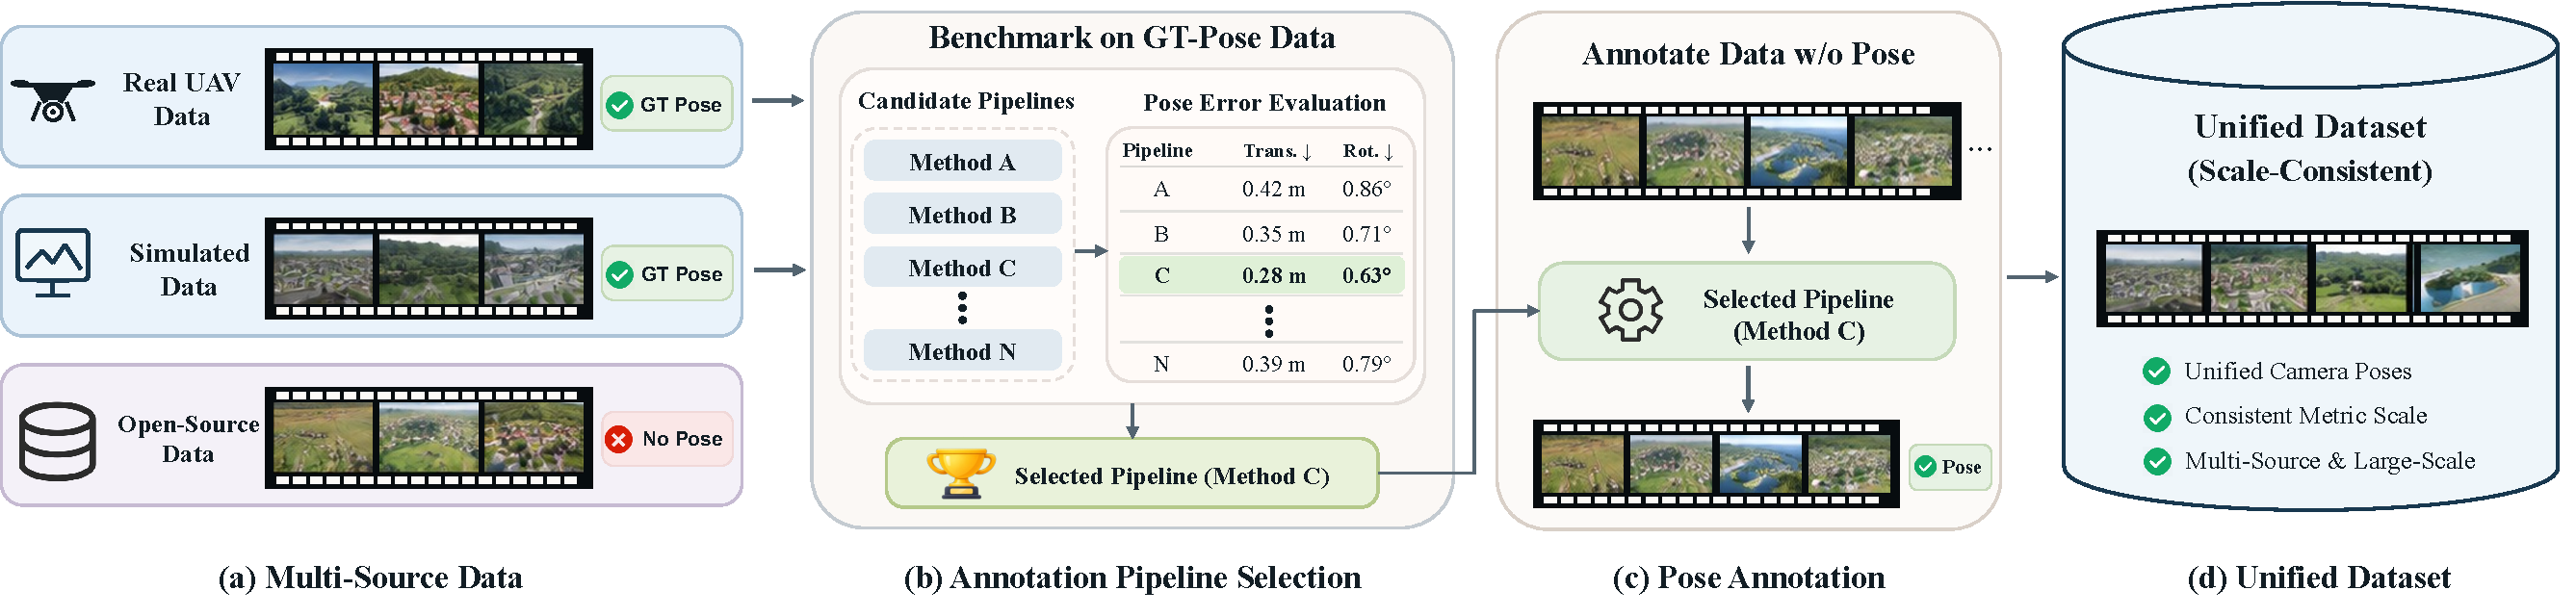
\includegraphics[width=\textwidth]{figures/data_pipeline.pdf}
    \caption{\textbf{Data construction and camera annotation.} (a) We collect complementary observations from real UAV flights, simulation, and open-source videos. (b) Simulator-recorded camera trajectories provide references for offline comparison of reconstruction accuracy, coverage, runtime, and translation scale. The selected pipeline initializes geometry with Pi3X, refines it through shared-intrinsics bundle adjustment, and recovers one scale per clip using calibrated UniDepthV2 predictions at reliable reconstructed points. (c) With the configuration fixed, videos without camera labels are annotated from RGB alone, without requiring reference poses at inference. (d) The resulting approximately metric annotations are combined with simulator reference geometry and real-flight observations to form the training corpus.}
    \label{fig:data_pipeline}
\end{figure*}

\begin{figure*}[t]
    \centering
    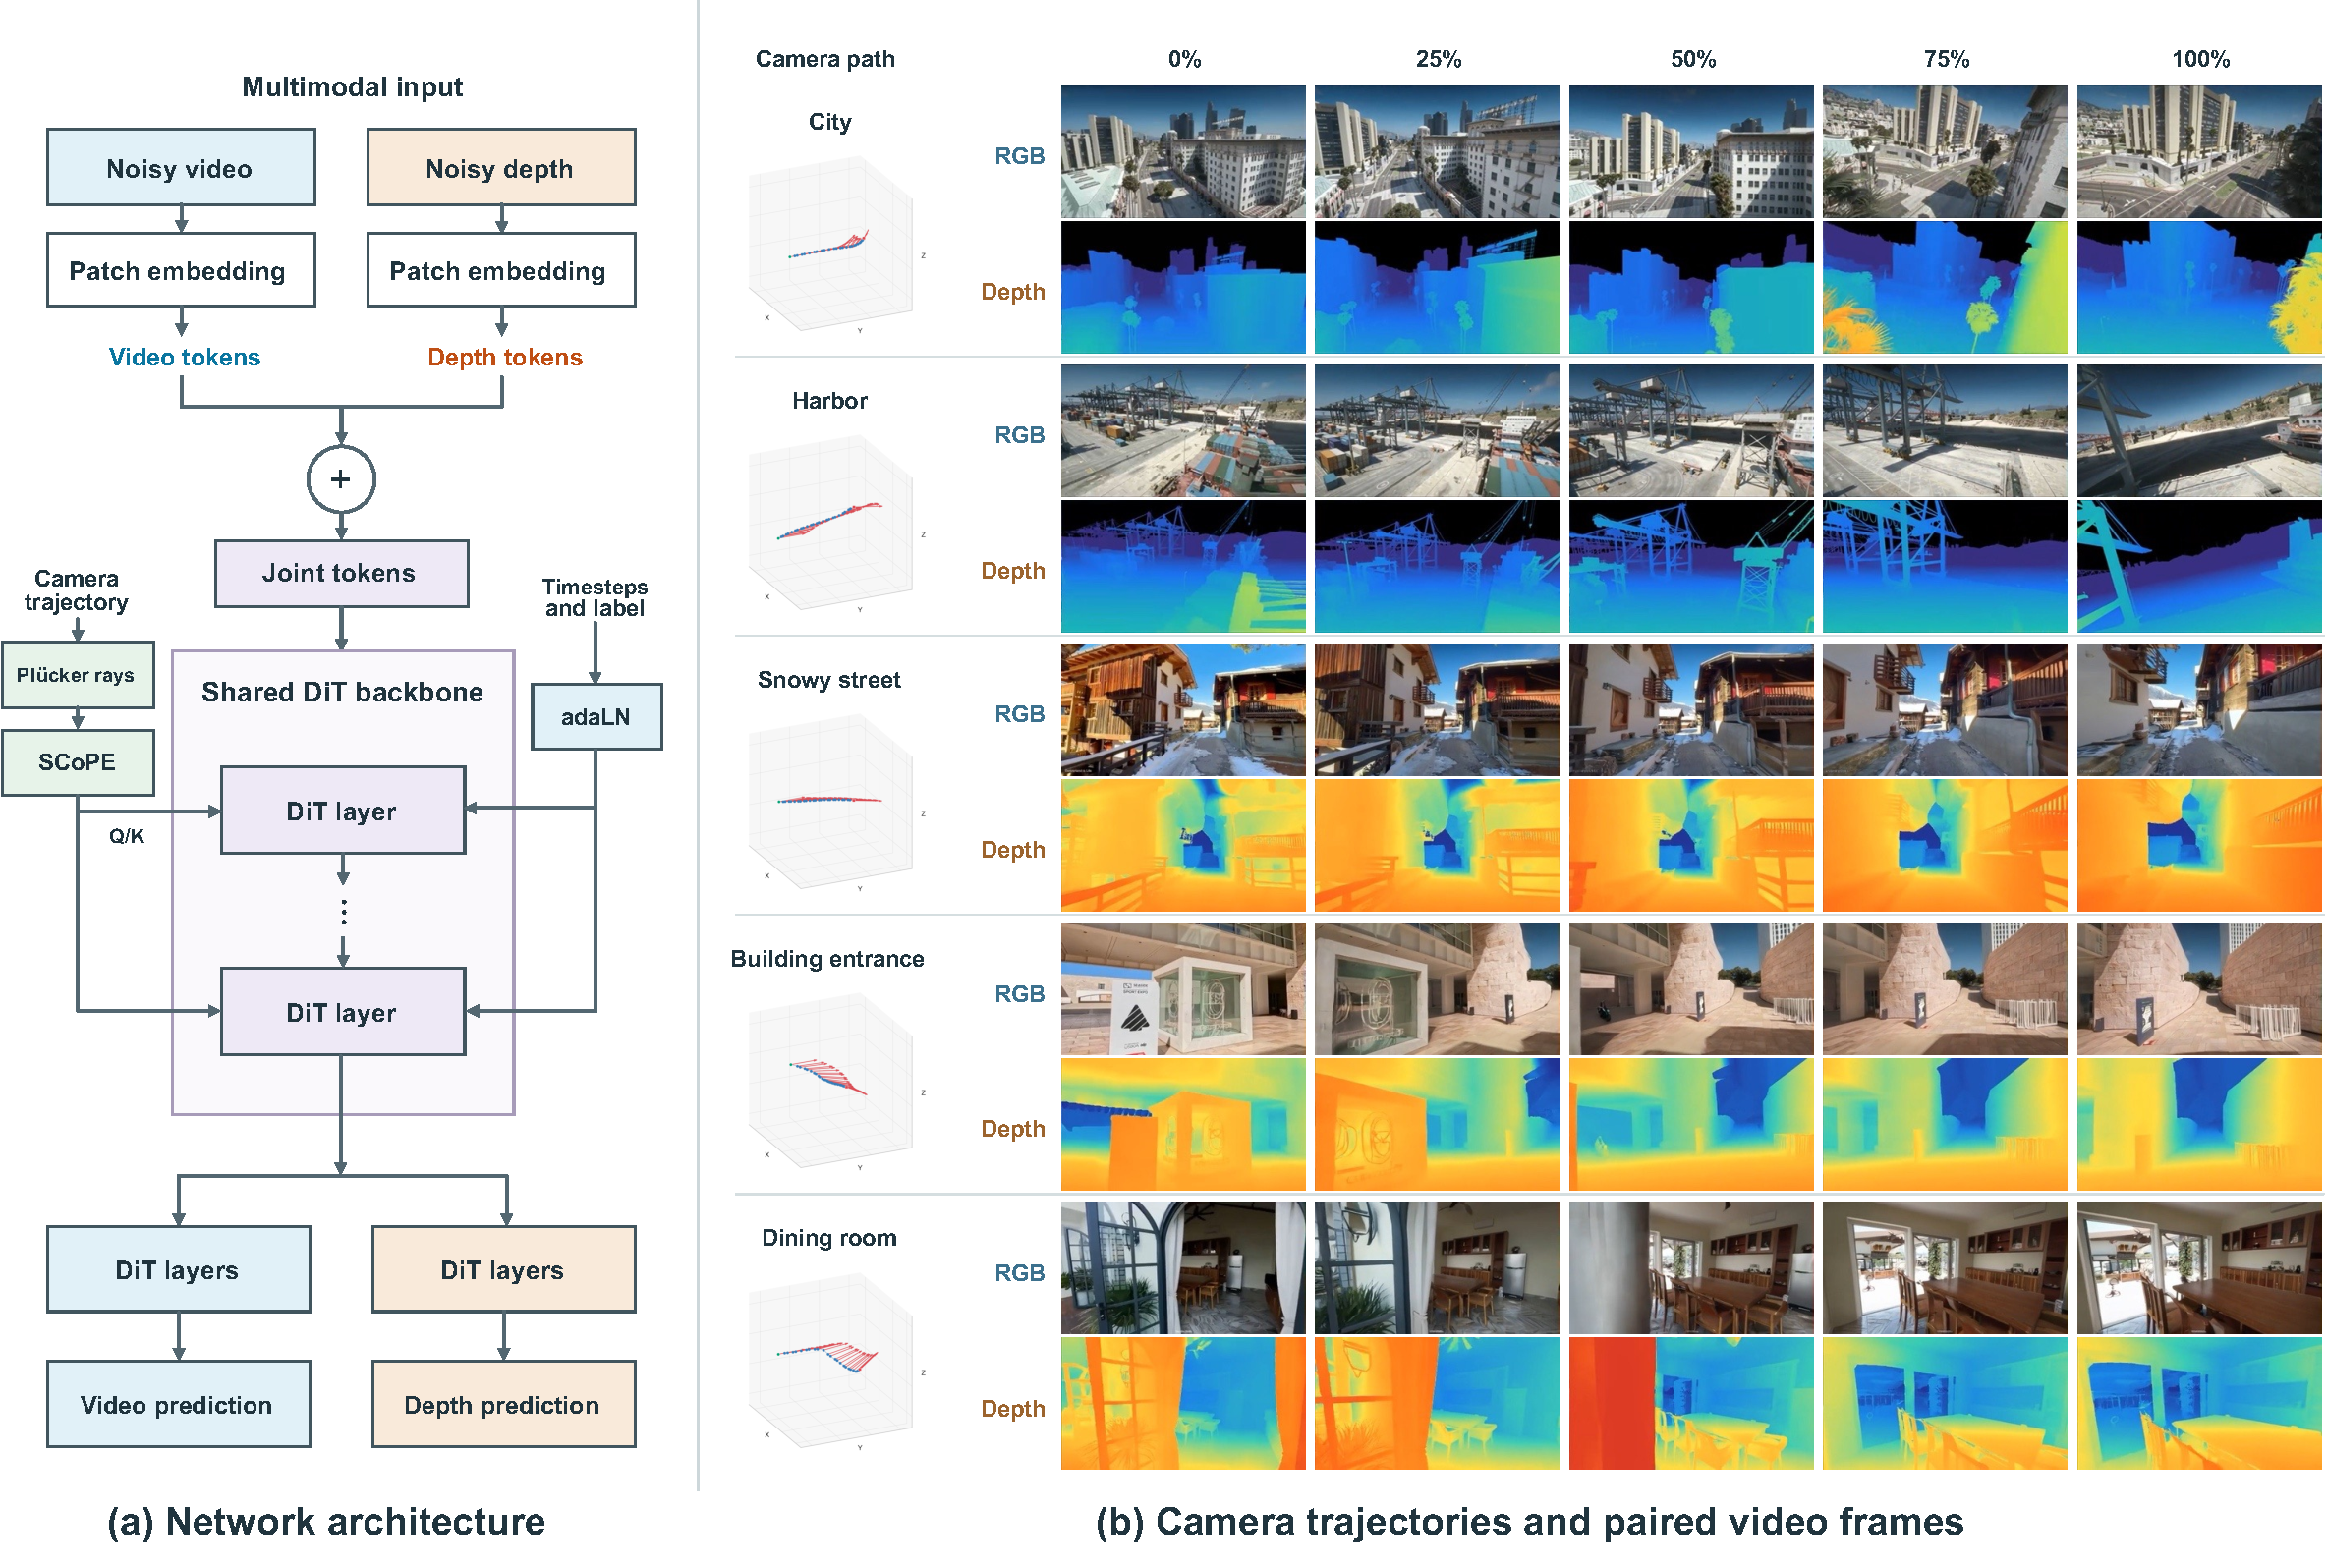
\includegraphics[width=\textwidth]{figures/method.pdf}
    \caption{\textbf{Camera-conditioned joint RGB--depth generation.} (a) Separate patch embeddings map noisy RGB and depth latents into tokens, which are concatenated and processed by a shared DiT backbone to exchange appearance and geometry information. Camera trajectories are represented as Pl\"ucker rays and injected into attention queries and keys through SCoPE, while timestep and label conditions modulate features through adaLN. The shared backbone then splits into modality-specific DiT branches for RGB and depth prediction. (b) Paired RGB and depth outputs at five trajectory positions illustrate viewpoint changes and corresponding scene structure across outdoor and indoor environments, with depth maps outlining foreground objects and distant scene geometry throughout the displayed camera motion.}
    \label{fig:method}
\end{figure*}

% !TeX root = ../main.tex
\section{Related Work}
\label{sec:related_work}

\subsection{Camera-Controllable Visual World Models}
\label{sec:rw_camera_models}

Camera-controllable visual world models generate future observations in response to viewpoint changes, enabling sequential exploration of a visual environment.
Earlier camera-conditioned generators, including MotionCtrl~\cite{wang2024motionctrlunifiedflexiblemotion}, CameraCtrl~\cite{he2025cameractrlenablingcameracontrol}, and CamCo~\cite{xu2024camcocameracontrollable3dconsistentimagetovideo}, establish pose-based control over video synthesis.
Interactive systems extend this capability to ongoing user control: Matrix-Game~2.0~\cite{he2026matrixgame20opensourcerealtime} injects keyboard and mouse actions into streaming generation, while Yume~\cite{mao2025yumeinteractiveworldgeneration} maps keyboard inputs to quantized camera motions for world exploration.
WorldPlay~\cite{sun2026worldplaylongtermgeometricconsistency} and LingBot-World~\cite{robbyantteam2026advancingopensourceworldmodels} further address scene persistence over longer interactive rollouts through mechanisms that retain historical context.
Aerial applications introduce flight-specific observations and controls, as explored by AirScape~\cite{zhao2025airscapeaerialgenerativeworld} and Aerial World Model~\cite{zhang2026aerialworldmodellonghorizon}.

Recent open systems address the inference cost and implementation complexity of long-horizon world modeling.
Efficiency-oriented models, including SANA-WM~\cite{zhu2026sanawmefficientminutescaleworld}, Wonder~\cite{xu2026wondervideoworldmodel}, and ABot-World-0~\cite{jiang2026abotworld0infiniteinteractiveworld}, reduce the computational cost of interactive generation through efficient attention, selective history access, or optimized streaming execution.
Complementing these model-level advances, minWM~\cite{zhao2026minwmfullstackopensourceframework}, BiWM~\cite{rui2026biwmadvancingopensourceinteractive}, and SolarWM~\cite{huang2026solarwmopendatascalable} provide reusable frameworks that organize camera-control adaptation, training, and inference into pipelines supporting multiple video backbones.

Alongside these advances in efficiency and system design, joint appearance and depth modeling has been explored for camera-conditioned generation.
Aether~\cite{zhu2025aethergeometricawareunifiedworld} jointly learns geometric reconstruction, video prediction, and visual planning.
DualCamCtrl~\cite{zhang2025dualcamctrldualbranchdiffusionmodel} couples parallel RGB and depth diffusion branches through semantic-guided mutual alignment, using an estimated initial depth map in its image-conditioned formulation.
IDCNet~\cite{liu2025idcnetguidedvideodiffusion} combines metric-aligned training data with joint RGB-depth generation conditioned on initial RGB-depth observations and camera trajectories.
Our focus is few-step causal RGB-depth generation for low-altitude flight from an initial RGB frame, text, and a camera trajectory.
We exchange appearance and geometry information through shared early transformer layers before modality-specific prediction, and supervise decoded depth with pixelwise log-depth and temporal-block scale losses.
This metric supervision is retained during causal adaptation, connecting joint geometry learning to sequential RGB-depth generation.

\subsection{Camera-Annotated Video Data}
\label{sec:rw_camera_data}

Camera-controlled generation depends on video data that associates observations with camera motion.
DL3DV-10K~\cite{ling2024dl3dv10klargescalescenedataset} provides diverse scene captures with reconstructed camera parameters, while Sekai~\cite{li2025sekaivideodatasetworld} combines real walking and drone videos with estimated trajectories and game videos with engine-recorded camera poses.
RealCam-Vid~\cite{zheng2025realcamvidhighresolutionvideodataset} reconstructs camera motion in dynamic scenes and aligns its scale using metric-depth predictions, while SpatialVID~\cite{wang2025spatialvidlargescalevideodataset} provides estimated poses and depth together with derived motion instructions.
Combining such sources requires reconciling their camera conventions, translation scales, and annotation procedures.

SolarWM~\cite{huang2026solarwmopendatascalable} standardizes heterogeneous sources into frame-aligned video, camera, caption, and quality records.
SANA-WM~\cite{zhu2026sanawmefficientminutescaleworld} builds metric camera annotations using temporally consistent geometry estimation and monocular metric-depth predictions.
Both pipelines accommodate existing camera or depth annotations, while their video-only branches recover metric geometry through estimation.
Our data construction combines simulation, public videos, and real UAV footage, using exact metric trajectories from simulation to calibrate scale recovery and compare pose estimators against ground truth.
The selected annotation procedure is then applied to recover camera trajectories from unannotated videos in a common metric convention.

\subsection{Autoregressive Video Generation}
\label{sec:rw_autoregressive}

Autoregressive video generation produces successive frames or temporal blocks conditioned on prior observations.
Diffusion Forcing~\cite{chen2024diffusionforcingnexttokenprediction} trains causal models with independently sampled noise levels across tokens, connecting next-token prediction with sequence diffusion.
CausVid~\cite{yin2025slowbidirectionalfastautoregressive} distills a bidirectional diffusion teacher into a few-step causal generator.
Self Forcing~\cite{huang2025selfforcingbridgingtraintest} trains on self-generated histories and applies distribution supervision, addressing the mismatch between reference histories during training and generated histories at inference.

Interactive world models adopt different training strategies to support camera-controlled autoregressive generation.
SolarWM~\cite{huang2026solarwmopendatascalable} uses bidirectional adaptation, teacher-forced autoregressive initialization, and distribution matching distillation as three successive training stages.
BiWM~\cite{rui2026biwmadvancingopensourceinteractive} retains bidirectional attention over the current chunk and visible history while generating chunks sequentially, using control fine-tuning followed by few-step distillation.
Direct Forcing~\cite{xu2026directforcingsinglestagetraining} instead combines future-frame feature alignment under reference histories with feature-space distribution matching under self-generated histories in one causal training stage.
Following this training formulation, we extend continuation alignment and rollout distribution matching to both RGB and depth while retaining decoded metric-depth supervision, adapting the joint model directly from bidirectional learning to few-step causal generation.

% !TeX root = ../main.tex
\section{Data Collection}
\label{sec:data}

Our training corpus combines real-world data collection, captures from a simulated environment, and open-source datasets (Fig.~\ref{fig:data_pipeline}).
The corpus contains 600,000 clips, including 200,000 simulation clips, and provides complementary observations, scene diversity, and geometric supervision.

\subsection{Data Sources}
\label{sec:data_sources}

\paragraph{Real-world data collection.}
We record onboard videos during real-world UAV flights, capturing observations under physical flight conditions.
We supplement these recordings with YouTube drone videos to expand the diversity of real-world aerial footage.

\paragraph{Simulation data collection.}
We build an automated collection pipeline in GTA V with DLSS 5 neural rendering~\cite{nvidia2026dlss5} to capture first-person UAV flights close to the ground.
An obstacle-avoiding flight controller supports continuous collection, while randomized turns diversify the trajectories.
We jointly export video, real-time camera poses, and linear depth maps derived from the rendering engine's depth buffers and aligned with the enhanced RGB frames.
The annotations share the simulator's approximately metre-scale units.
The combination of realistic imagery and accurate camera and depth annotations makes this our highest-quality source for geometric supervision.

\paragraph{Open-source datasets.}
We use Sekai-Walking-Clean and SpatialVID-Clean from SolarWM~\cite{huang2026solarwmopendatascalable}, derived from Sekai~\cite{li2025sekaivideodatasetworld} and SpatialVID~\cite{wang2025spatialvidlargescalevideodataset}, retaining only the \texttt{high} and \texttt{xhigh} quality tiers.
These clips are filtered and processed using distilled LTX-2.3-22B with the Clean Plate IC-LoRA adapter to remove people and vehicles.
We also include the drone subset of Sekai for additional aerial observations.
% Model identity verified against SolarWM Sec. 5.3 and its released manifest:
% https://arxiv.org/html/2609.02886v1#S5.SS3
% https://github.com/Enderfga/solarwm-data/blob/main/configs/clean_plate_models.json

From DL3DV-10K~\cite{ling2024dl3dv10klargescalescenedataset}, we reconstruct scenes with 3D Gaussian Splatting (3DGS) and render videos along designed camera trajectories.
We apply Difix3D+~\cite{wu2025difix3d} to repair dark patches and streaking artifacts, then use optical-flow correspondences between successive frames for temporal smoothing to reduce flicker.

\subsection{Camera Annotation}
\label{sec:camera_annotation}

For videos without camera labels, Pi3X~\cite{wang2026pi3permutationequivariantvisualgeometry} initializes poses and scene geometry, followed by bundle adjustment (BA) with shared intrinsics.
We align UniDepthV2~\cite{piccinelli2025unidepthv2} predictions with reliable reconstructed points and apply bounded inverse-depth correction to recover one positive scale per clip, preserving rotations and trajectory shape.
Section~\ref{sec:annotation_evaluation} presents the selection evidence, and the Supplementary Material gives implementation details.

\subsection{Depth Annotation}
\label{sec:depth_annotation}

For non-GTA videos, MetricAnything Student PointMap~\cite{ma2026metricanything} provides approximately metric optical-axis depth.
Metric Video Depth Anything (VDA) Large~\cite{chen2025videodepthanything} stabilizes framewise scale while preserving spatial structure.
We temporally stabilize sky masks from Depth Anything 3~\cite{lin2025depthanything3}, then downsample depth and apply the shared logarithmic encoding in Sec.~\ref{sec:bidirectional_training}.
Section~\ref{sec:annotation_evaluation} summarizes GTA validation, and the Supplementary Material details alignment and sky processing.

% Depth implementation verified against AutoDL's deployed metric_depth_models.py,
% metric_depth_processing.py, metric_depth_contract.py, and source-config.local.json
% under df-full-20261102, plus the GTAAligned depth-cache metadata.

% !TeX root = ../main.tex
% Revised 2026-11-05: two stages, following the author's updated training recipe.
\section{Method}
\label{sec:method}

Our model is trained in two stages to generate paired RGB observations and depth maps along prescribed camera trajectories (Fig.~\ref{fig:method}).
The first stage learns camera-conditioned generation with bidirectional attention, using joint depth prediction to improve the geometric consistency of generated videos and their adherence to prescribed camera trajectories (Sec.~\ref{sec:bidirectional_training}).
The second stage directly converts the bidirectional multi-step model into a few-step causal generator through supervised causal continuation under teacher forcing and feature-space distribution matching under self forcing (Sec.~\ref{sec:causal_adaptation}).

\subsection{Bidirectional camera-control training}
\label{sec:bidirectional_training}
\label{sec:joint_generation}


We build on Wan2.2-TI2V-5B~\cite{wan2025wanopenadvancedlargescale} to jointly predict future RGB frames and full-clip depth, conditioned on $\mathbf c=(I_0,y,\mathcal{C})$.
%
Here, $I_0$ is the initial RGB frame, $y$ is the text condition, and $\mathcal{C}=\{(K_t,P_t)\}_{t=0}^{T}$ specifies the camera intrinsics and poses along the trajectory.
%
For metric ground-truth adaptation, we spatially downsample optical-axis depth $D$ in metric space and apply logarithmic normalization to map valid depths into $[-1,1]$:
\begin{equation}
\begin{aligned}
D_{\mathrm{clip}} &= \min(\max(D,a),b),\\
g(D) &= 2\frac{\log(D_{\mathrm{clip}}/a)}{\log(b/a)}-1,
\end{aligned}
\label{eq:metric_depth_encoding}
\end{equation}
where $a=0.1$\,m and $b=2000$\,m define fixed depth bounds shared across all samples.

%
The mapped depth, with invalid regions filled, is replicated into three channels and encoded using the same frozen Wan VAE as RGB.
%
The first 24 transformer layers are shared by RGB and depth, allowing their concatenated tokens to exchange appearance and geometry information through bidirectional attention.
%
The shared layers are followed by separate RGB and depth prediction branches, each comprising six transformer layers.
%
Both modalities are jointly trained with linear flow matching.
%
For each modality $m\in\{\mathrm{rgb},\mathrm{dep}\}$, let $z_0^m$ denote its clean VAE latent, $\epsilon^m$ independently sampled Gaussian noise, and $\sigma_m$ its noise level.
%
Given the joint noisy latents $\mathbf z_{\boldsymbol\sigma}$ and noise conditions $\boldsymbol\sigma$, the model predicts $v_\theta^m=f_\theta^m(\mathbf z_{\boldsymbol\sigma},\boldsymbol\sigma,\mathbf c)$.
%

For each modality $m\in\{\mathrm{rgb},\mathrm{dep}\}$, we construct the noisy latent $z_{\sigma_m}^{m}=(1-\sigma_m)z_0^{m}+\sigma_m\epsilon^{m}$, with target velocity $v^{m,*}=\epsilon^{m}-z_0^{m}$.
%
The joint flow-matching objective is defined as
\begin{equation}
\mathcal{L}_{\mathrm{FM}}
=\sum_m\mathbb{E}\!\left[
\operatorname{MSE}(v_\theta^m,v^{m,*})
\right].
\label{eq:joint_flow_matching}
\end{equation}


To further enforce metric depth accuracy and scale consistency, we introduce additional supervision on the decoded depth predictions.
%
Specifically, the clean depth latent is estimated as
\begin{equation}
\widehat z_0^{\mathrm{dep}}
=z_{\sigma_{\mathrm{dep}}}^{\mathrm{dep}}
-\sigma_{\mathrm{dep}}v_{\theta}^{\mathrm{dep}},
\label{eq:clean_depth_estimate}
\end{equation}
which is decoded through the frozen VAE and mapped by $g^{-1}$ to metric depth $\widehat D$.
%
For valid pixels $i\in\Omega$ in a sampled temporal block with $0<\sigma_{\mathrm{dep}}\leq0.8$, let $\delta_i=\log\widehat D_i-\log D_i$.
%
We define
\begin{equation}
\begin{aligned}
\mathcal{L}_{\mathrm{abs\text{-}log}}
&=\frac{1}{|\Omega|}\sum_{i\in\Omega}|\delta_i|,\\
\mathcal{L}_{\mathrm{chunk\text{-}scale}}
&=\left(\frac{1}{|\Omega|}\sum_{i\in\Omega}\delta_i\right)^2.
\end{aligned}
\label{eq:decoded_depth_losses}
\end{equation}
These terms penalize pixelwise log-depth errors and blockwise scale bias, respectively.
%
We combine them into a metric depth loss $\mathcal{L}_{\mathrm{metric}}=\lambda_{\mathrm{metric}}(\mathcal{L}_{\mathrm{abs\text{-}log}}+\mathcal{L}_{\mathrm{chunk\text{-}scale}})$, with $\lambda_{\mathrm{metric}}=0.05$.
%
The bidirectional objective is
\begin{equation}
\mathcal{L}_{\mathrm{bi}}=\mathcal{L}_{\mathrm{FM}}+\mathcal{L}_{\mathrm{metric}}.
\label{eq:bidirectional_objective}
\end{equation}

Complementary to the output-level depth supervision, we adopt SCoPE~\cite{yin2026scope} to incorporate explicit camera geometry into self-attention.
%
Specifically, SCoPE encodes each token's camera ray as a positional feature and adds it only to the attention queries and keys, while preserving the original RoPE.
%
This enables attention to capture geometric relationships across viewpoints, improving camera controllability and cross-frame geometric consistency.


\subsection{Direct training for few-step causal generation}
\label{sec:causal_adaptation}

We adapt the camera-controllable bidirectional RGB--Depth model to causal generation to support sequential prediction and interaction in world models.
%
Following Direct Forcing~\cite{xu2026directforcingsinglestagetraining}, we adopt block-causal temporal attention and extend Causal Continuation Alignment (CCA) and Rollout Distribution Matching (RDM) to joint RGB--Depth generation, enabling few-step autoregressive generation.

For CCA, the model predicts clean RGB and depth latents from noisy current chunks conditioned on clean reference histories.
%
We employ frozen VideoMAE encoders $\psi^m$ to align the decoded predictions $\widetilde{x}^m$ with their references $x^m$ through a cosine feature loss:
\begin{equation}
\mathcal{L}_{\mathrm{CCA}}^m
=\mathbb{E}\left[
\mathcal{D}_{\mathrm{cos}}\left(
\psi^m(\widetilde{x}^m),
\operatorname{sg}(\psi^m(x^m))
\right)\right],
\label{eq:causal_cca}
\end{equation}
where $m\in\{\mathrm{rgb},\mathrm{dep}\}$ and $\mathcal{D}_{\mathrm{cos}}$ denotes the token-wise cosine feature distance.

To account for errors accumulated during autoregressive generation, RDM matches the distributions of self-generated rollouts and reference videos.
%
We employ three representation spaces $\mathcal{E}=\{\mathrm{RGB\text{-}Cosmos},\mathrm{RGB\text{-}VideoMAE},\mathrm{Depth\text{-}VideoMAE}\}$, each combining visual and text features as $h_e(x,y)=[\phi_e(x),\beta_e t(y)]$.
%
For each space $e$, we measure the discrepancy between generated and reference distributions using squared maximum mean discrepancy (MMD) with a Gaussian kernel $k_e$, denoted by $\mathcal{D}_e=\operatorname{MMD}_{k_e}^2(\mathcal{P}_\theta^e,\mathcal{Q}^e)$.
%
We construct the reference distribution from 8192 fixed training samples and approximate its kernel mean using 4096 Nystr\"om landmarks.
%
The resulting empirical discrepancies are normalized and equally weighted:
\begin{equation}
\mathcal{L}_{\mathrm{RDM}}
=\mathbb{E}_{e\sim\mathcal{U}(\mathcal{E})}
\left[
\frac{\widehat{\mathcal{D}}_e}
{\operatorname{sg}(|\widehat{\mathcal{D}}_e|)+\varepsilon}
\right].
\label{eq:causal_rdm}
\end{equation}


To preserve metric depth accuracy during causal generation, we retain $\mathcal{L}_{\mathrm{metric}}$ from the bidirectional training stage.
%
The overall post-training objective is
\begin{equation}
\mathcal{L}_{\mathrm{post}}
=\mathcal{L}_{\mathrm{RDM}}
+\operatorname{sg}(\lambda_t)
\mathcal{L}_{\mathrm{CCA}}+\mathcal{L}_{\mathrm{metric}},
\label{eq:causal_objective}
\end{equation}
where $\mathcal{L}_{\mathrm{CCA}}$ is the mean of the RGB and depth CCA losses, and $\lambda_t$ dynamically balances the RDM and paired-supervision gradients based on the relative CCA residuals and gradient norms.
%
By combining distribution matching, continuation alignment, and metric depth supervision, this training strategy enables coherent autoregressive RGB-Depth generation while preserving geometric consistency.




% !TeX root = ../main.tex
\section{Experiments}
\label{sec:experiments}
\setcounter{dbltopnumber}{2}

\subsection{Experimental setup}
\label{sec:experiment_setup}

We initialize our model from Wan2.2-TI2V-5B and train with BF16 precision, keeping the VAE and text encoder frozen.
Training clips contain 81 frames at 16\,fps, with RGB resolution $832\!\times\!480$ and depth resolution $448\!\times\!256$.
We train the bidirectional model for 2 epochs with a batch size of 64, followed by 250 steps of causal post-training with a batch size of 256.

We select subsets from multiple data sources, yielding 1,350 evaluation clips in total.
Each clip contains 81 frames at 16\,fps.

We compare with text-and-image-to-video (TI2V) world models: SolarWM-5B SGF Stage~2~\cite{huang2026solarwmopendatascalable} and the Hunyuan DMD variant of minWM~\cite{zhao2026minwmfullstackopensourceframework}.
All compared models generate videos conditioned on an initial RGB frame, a text prompt, and a camera trajectory through their native conditioning interfaces.
For the quantitative comparison, our model and SolarWM use four denoising steps at $832\!\times\!480$ and $864\!\times\!480$, respectively; pixel-level references follow the corresponding native preprocessing.
For minWM, we retain its native camera-translation normalization.
% Evaluated weights: our DF step252 raw checkpoint; official SolarWM Stage2 EMA.
% minWM results come from the author-supplied three-model-metrics.json.
% The matching minWM full-scaled outputs and ViPE summary were verified on
% AutoDL; per-clip translation normalization is retained in those outputs.

For visual fidelity, we report LPIPS with AlexNet features~\cite{zhang2018lpips} and FVD~\cite{unterthiner2018fvd}.
LPIPS excludes the conditioning frame, with equal weighting across clips.
FVD uses all 81 frames and a shared 400-dimensional pre-softmax I3D representation at $224\!\times\!224$ resolution.

For camera control, ViPE~\cite{huang2025vipevideoposeengine} recovers trajectories from generated RGB, independently of our predicted depth.
We report SCoPE's framewise RotErr (degrees), TransErr, and CamMC~\cite{yin2026scope}, supplemented by pose-matrix cosine similarity (CosSim) and all-pairs relative-pose AUC at $15^\circ$/$30^\circ$~\cite{wang2025vggt}.
Trajectories are anchored at the first frame and translations independently normalized by maximum displacement; these scores assess relative motion rather than absolute scale.

\subsection{Annotation pipeline evaluation}
\label{sec:annotation_evaluation}

Conventional SfM and learning-based estimators offer several routes to camera annotation, but reference trajectories are generally unavailable for web videos.
Our camera-pipeline validation uses 16 clips, comprising 12 GTA clips and four real-world clips.
The simulator provides diverse scenes, realistic imagery, and recorded trajectories, enabling comparisons of reconstruction quality, runtime, and scale recovery.
We first compare reconstruction strategies and then examine scale accuracy to select the hybrid pipeline in Sec.~\ref{sec:camera_annotation}.

\paragraph{Reconstruction and scale.}
Table~\ref{tab:pose_coverage} compares SIFT and LightGlue with COLMAP against Pi3X initialized reconstruction with shared-intrinsics BA.
Pi3X produces complete outputs for all 16 clips in a median of 26.69 seconds, compared with 140.86 seconds for SIFT and 94.71 seconds for LightGlue.
SIFT has the lowest median ATE on the common valid subset, while Pi3X has the lowest P90 error.
The higher cost of conventional SfM therefore yields inconsistent accuracy gains, motivating learned initialization for large-scale annotation.

\begin{table}[htbp]
    \centering
    \caption{SfM versus learned reconstruction. Complete outputs and median runtime use all 16 clips. Sim3 ATE is camera-center RMSE in reference-trajectory units on seven common valid clips.}
    \label{tab:pose_coverage}
    \small
    \setlength{\tabcolsep}{3pt}
    \begin{tabular}{lrrr}
        \toprule
        Method & Full & Time (s) $\downarrow$ & \shortstack{ATE $\downarrow$\\median / P90} \\
        \midrule
        SIFT + COLMAP & 10/16 & 140.86 & \textbf{0.04125} / 1.40108 \\
        LightGlue + COLMAP & 13/16 & 94.71 & 0.88925 / 4.47273 \\
        Pi3X + BA & \textbf{16/16} & \textbf{26.69} & 0.06356 / \textbf{0.10589} \\
        \bottomrule
    \end{tabular}
\end{table}

Among learned methods, Pi3X and ViPE~\cite{huang2025vipevideoposeengine} both recover accurate relative geometry after scale alignment (Table~\ref{tab:learned_geometry}).
Their median normalized ATE is 0.083--0.127\% and rotation error is approximately $0.46^\circ$, while scale errors remain 20.64--22.17\% under a common UniDepthV2 backend.
We retain Pi3X for its complete-frame coverage and focus further comparison on translation scale, which determines the magnitude of camera-motion supervision.
Native Pi3X alone has a 38.87\% median scale error on an eight-clip ablation subset, motivating the additional geometric refinement and calibrated scale recovery detailed in the Supplementary Material.

\begin{table}[htbp]
    \centering
    \caption{Relative geometry and scale. Error medians use 14 common successful clips. Sim3 ATE is normalized by reference path length, while coverage uses all 16 clips.}
    \label{tab:learned_geometry}
    \small
    \setlength{\tabcolsep}{3pt}
    \begin{tabular}{lrrrr}
        \toprule
        Geometry & Full & ATE (\%) $\downarrow$ & Rot. ($^\circ$) $\downarrow$ & Scale (\%) $\downarrow$ \\
        \midrule
        Pi3X + BA & \textbf{16/16} & 0.127 & 0.460 & 22.17 \\
        ViPE + BA & 14/16 & 0.125 & 0.459 & \textbf{20.64} \\
        ViPE, native & 14/16 & \textbf{0.083} & \textbf{0.455} & 21.30 \\
        \bottomrule
    \end{tabular}
\end{table}

\begin{table}[htbp]
    \centering
    \caption{Calibrated scale recovery with fixed geometry. Median and P90 scale errors use 15 scorable outputs from 16 attempted clips with frozen parameters.}
    \label{tab:scale_selection}
    \small
    \setlength{\tabcolsep}{3pt}
    \begin{tabular}{lrr}
        \toprule
        Scale configuration & Median (\%) $\downarrow$ & P90 (\%) $\downarrow$ \\
        \midrule
        UniDepthV2, P98 baseline & 25.46 & 51.65 \\
        + inverse-depth correction & \textbf{22.40} & \textbf{45.60} \\
        \bottomrule
    \end{tabular}
\end{table}

Holding geometry and intrinsics fixed, inverse-depth correction reduces median scale error from 25.46\% to 22.40\% and P90 from 51.65\% to 45.60\% (Table~\ref{tab:scale_selection}).
It achieves the lowest median error among the evaluated scale configurations, whose complete comparison appears in the Supplementary Material.
The remaining scale error highlights the importance of directly recorded camera trajectories and depth for geometric supervision, together with real-flight observations of the intended operating conditions.

\begin{table}[htbp]
    \centering
    \caption{Depth annotation on 16 GTA clips. AbsRel and RMSE use the 0.1--80\,m range. Temporal log-depth error uses motion-compensated correspondences over 0.1--1,000\,m. Lower is better.}
    \label{tab:depth_annotation_selection}
    \small
    \setlength{\tabcolsep}{3pt}
    \begin{tabular}{@{}lrrr@{}}
        \toprule
        Configuration & AbsRel (\%) & RMSE (m) & Temporal \\
        \midrule
        MetricAnything & \textbf{17.69} & \textbf{9.54} & 0.03759 \\
        + VDA stabilization & 18.20 & 9.63 & \textbf{0.02124} \\
        \bottomrule
    \end{tabular}
\end{table}

\begin{table*}[t]
    \centering
    \caption{Quantitative comparison with TI2V world models on 1,350 clips. We evaluate visual fidelity and camera-trajectory adherence, with camera control measured from ViPE-recovered RGB trajectories after per-clip translation normalization. Best results are bold.}
    \label{tab:main_comparison}
    \small
    \setlength{\tabcolsep}{6pt}
    \begin{tabular}{@{}lrrrrrrrr@{}}
        \toprule
        & \multicolumn{2}{c}{Visual fidelity} & \multicolumn{6}{c}{Camera control} \\
        \cmidrule(lr){2-3}\cmidrule(l){4-9}
        Method & LPIPS$\downarrow$ & FVD$\downarrow$ & RotErr$\downarrow$ & TransErr$\downarrow$ & CamMC$\downarrow$ & CosSim$\uparrow$ & AUC@15$\uparrow$ & AUC@30$\uparrow$ \\
        \midrule
        minWM & 0.515 & 302.63 & 12.132 & 0.299 & 0.453 & 0.942 & 0.141 & 0.333 \\
        SolarWM & 0.490 & 171.07 & 5.239 & 0.133 & 0.202 & 0.980 & 0.544 & 0.708 \\
        Ours & \textbf{0.373} & \textbf{51.75} & \textbf{1.945} & \textbf{0.090} & \textbf{0.111} & \textbf{0.991} & \textbf{0.695} & \textbf{0.813} \\
        \bottomrule
    \end{tabular}
\end{table*}

\begin{figure*}[!t]
    \centering
    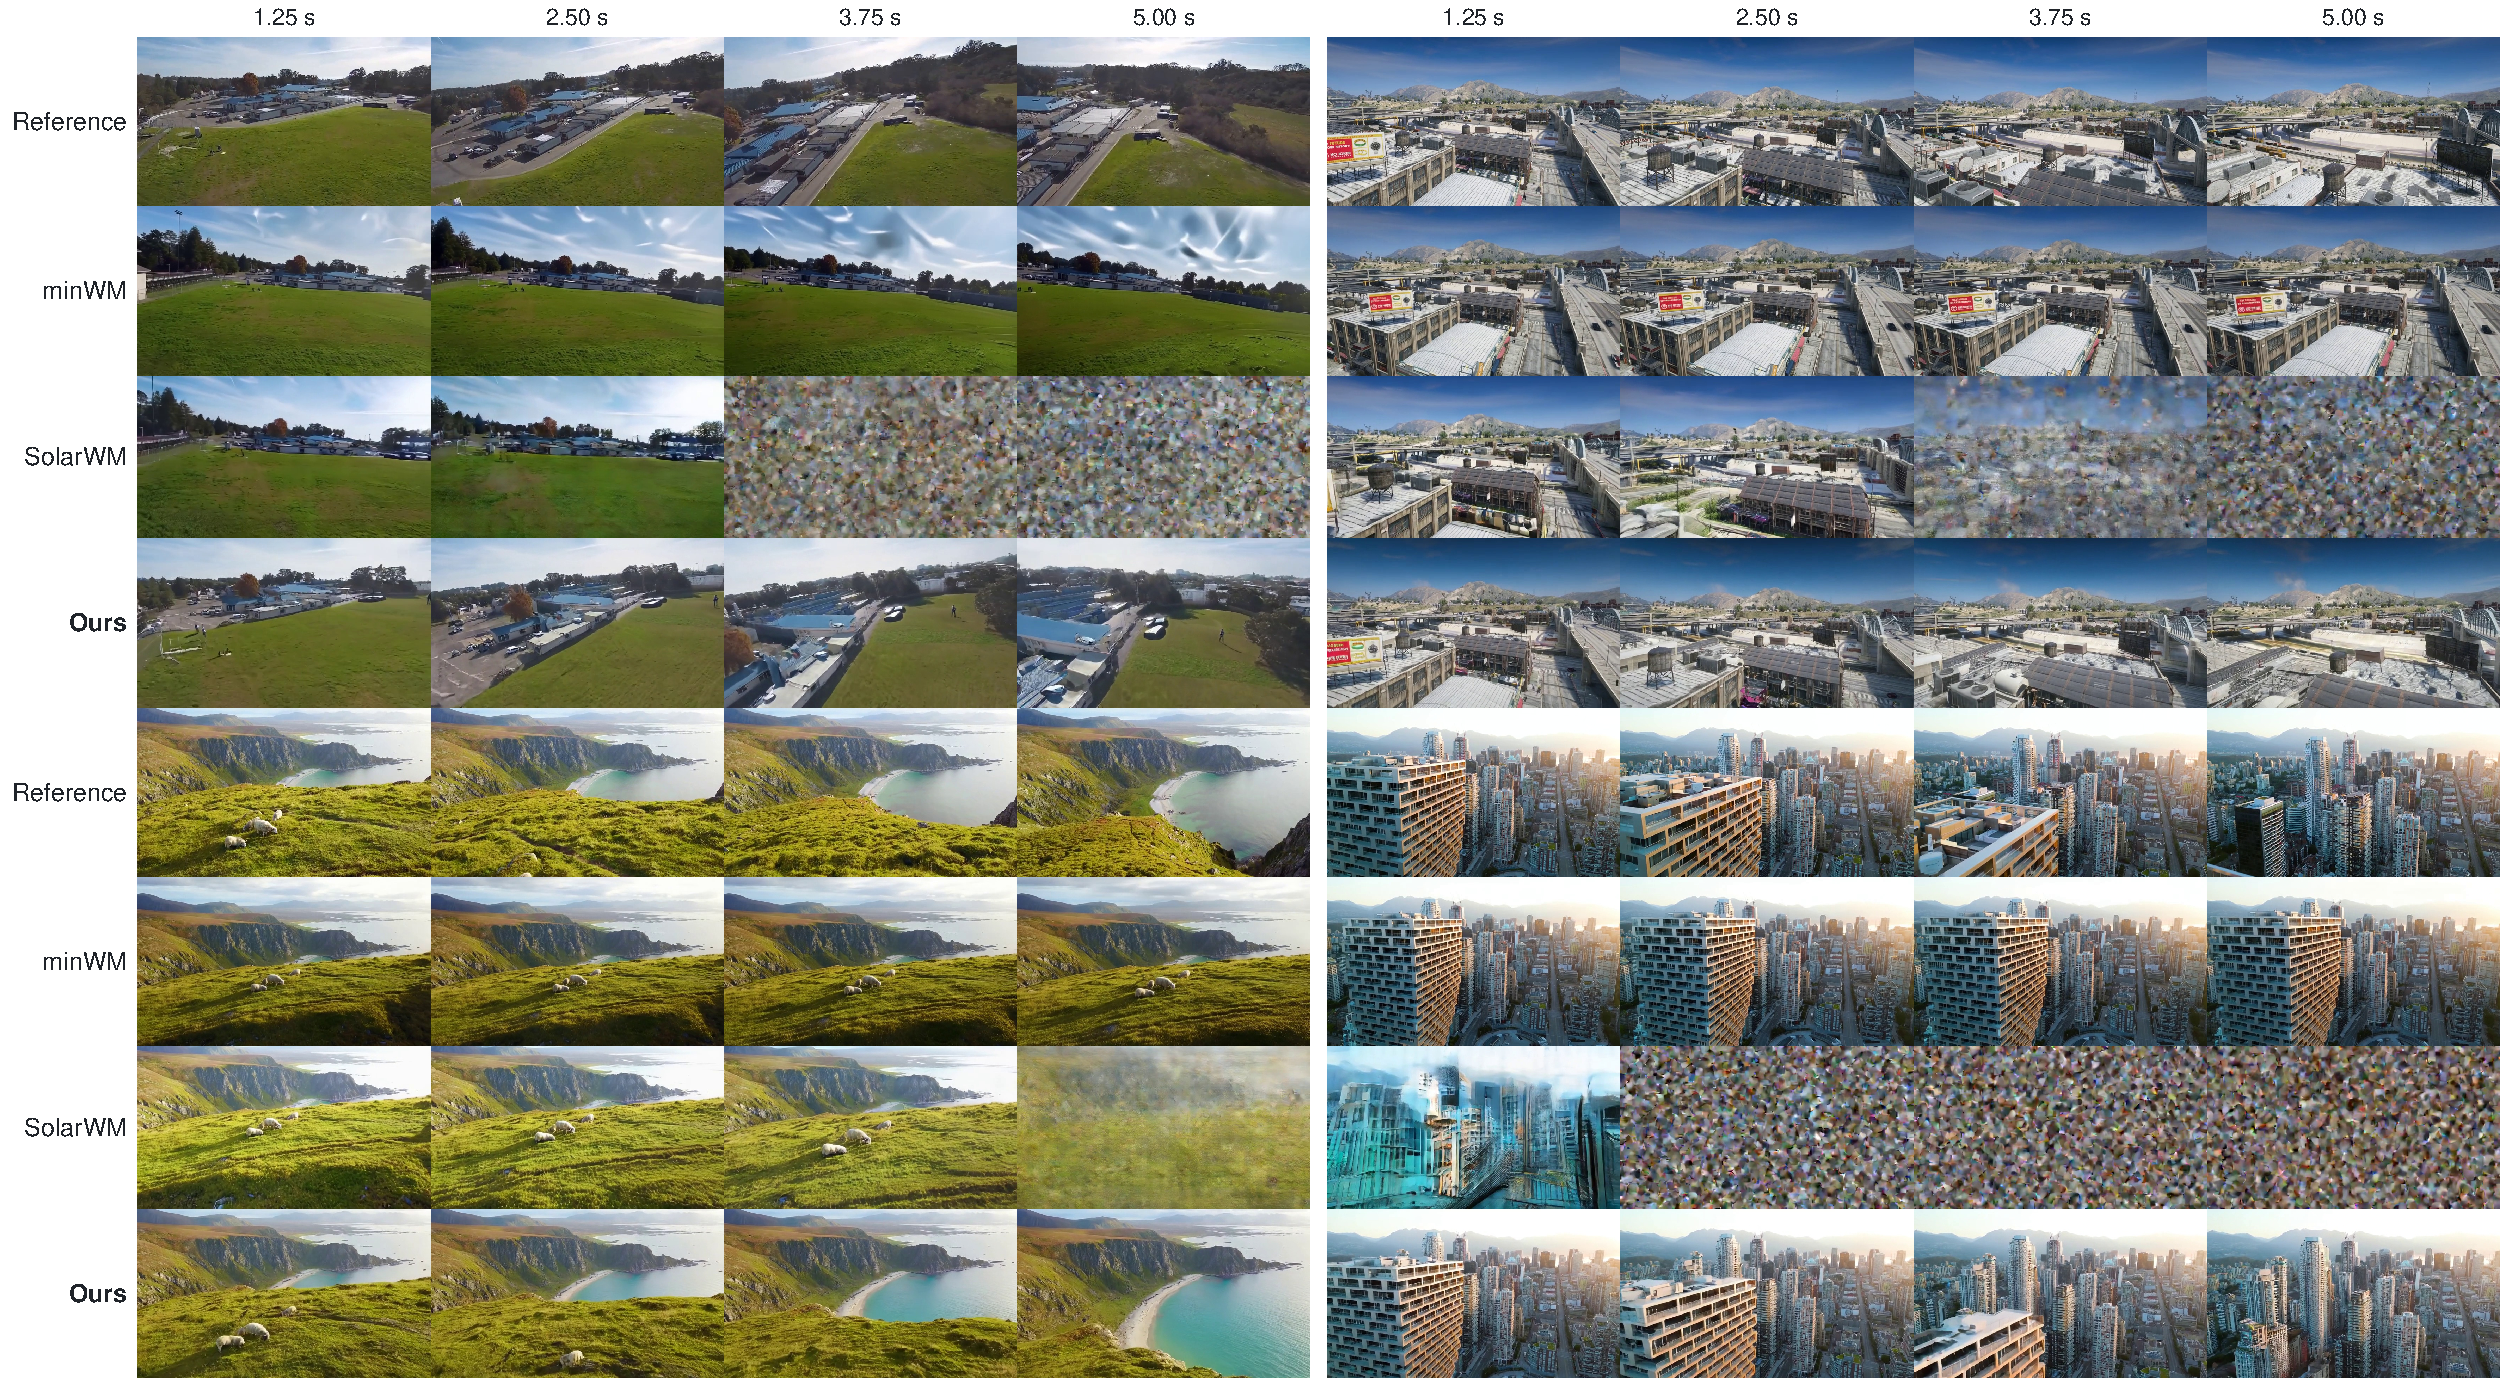
\includegraphics[width=\textwidth]{figures/qualitative_comparison.pdf}
    \caption{Qualitative comparison of camera-conditioned TI2V world models. The examples compare scene-structure preservation and viewpoint progression.}
    \label{fig:qualitative_comparison}
\end{figure*}

\paragraph{Depth accuracy and temporal consistency.}
We separately evaluate depth annotation on 16 GTA clips with reference depth, using all 81 frames per clip.
Table~\ref{tab:depth_annotation_selection} compares MetricAnything with the selected MetricAnything--VDA combination under RGB-only inference.
We average per-clip errors equally and measure temporal log-depth error along correspondences obtained from reference depth and camera motion.
VDA-guided stabilization reduces temporal error from 0.03759 to 0.02124, with AbsRel changing from 17.69\% to 18.20\% and RMSE from 9.54 to 9.63\,m.
The combination achieves the lowest temporal error among the evaluated configurations while maintaining similar per-frame depth accuracy.
The Supplementary Material includes the full focal-input comparison and evaluation protocol.

% Pose selection evidence: camera_trajectory_report.md, Sections 7.2, 7.3,
% 7.6, 7.7, and 7.9. Validation composition follows the author's correction
% to 12 GTA clips and four real-world clips. Common valid subsets are kept.
% Depth evidence: metric-depth-rgb-v1.0/evidence/nok_results.csv,
% protocol.json, and nok_protocol.json. This is a separate 16-GTA-clip panel.

\subsection{Quantitative comparison}
\label{sec:experiment_results}

Table~\ref{tab:main_comparison} shows that our model achieves the best scores across all reported metrics among the three evaluated checkpoints.
Compared with SolarWM, LPIPS decreases by 23.8\% and FVD by 69.7\%.

The visual gains are accompanied by more accurate camera control.
Relative to SolarWM, our model reduces rotation error by 62.9\% and normalized translation error by 32.6\%, while AUC@30 increases from 0.708 to 0.813.
Thus, on this evaluation panel, improved appearance is accompanied by closer adherence to the requested trajectory.
These comparisons evaluate complete systems; we examine the contribution of joint depth prediction separately in Sec.~\ref{sec:depth_ablation}.

\subsection{Depth ablation}
\label{sec:depth_ablation}

\begin{table}[t]
    \centering
    \caption{Depth ablation comparing RGB-only and joint RGB--depth generation. Appearance and camera-control metrics assess the contribution of depth supervision. Best results are bold.}
    \label{tab:depth_ablation}
    \small
    \setlength{\tabcolsep}{8pt}
    \begin{tabular}{@{}lrr@{}}
        \toprule
        Metric & RGB-only & RGB+Depth \\
        \midrule
        PSNR (dB)$\uparrow$ & 13.954 & \textbf{15.515} \\
        SSIM$\uparrow$ & 0.39115 & \textbf{0.43722} \\
        LPIPS$\downarrow$ & 0.40428 & \textbf{0.36595} \\
        FVD$\downarrow$ & 52.350 & \textbf{47.874} \\
        \midrule
        RotErr ($^\circ$)$\downarrow$ & 2.305 & \textbf{1.876} \\
        TransErr$\downarrow$ & 0.09501 & \textbf{0.08600} \\
        CamMC$\downarrow$ & 0.12069 & \textbf{0.10632} \\
        CosSim$\uparrow$ & 0.89129 & \textbf{0.99155} \\
        AUC@15$\uparrow$ & 62.26\% & \textbf{70.49\%} \\
        AUC@30$\uparrow$ & 72.98\% & \textbf{81.76\%} \\
        \bottomrule
    \end{tabular}
\end{table}

Table~\ref{tab:depth_ablation} compares RGB-only generation with joint RGB--depth generation to assess the contribution of depth prediction and supervision.
For this ablation, we additionally report PSNR and SSIM as complementary appearance metrics.
Joint generation improves both visual fidelity and camera control: LPIPS decreases by 9.5\%, rotation error by 18.6\%, and AUC@30 increases by 8.78 percentage points.
These results support joint depth prediction as useful geometric supervision for camera-conditioned video generation.

\subsection{Qualitative comparison}
\label{sec:qualitative_comparison}

% Selected scenes: 019, 021, 044, 066, 079, 093 in the author's review gallery.
% The Ours visualizations use step005427 live weights; the quantitative table
% retains the measured DF step252 results. The figure PDF is used unchanged.

Figure~\ref{fig:qualitative_comparison} shows six selected examples from real and simulated scenes.
In these examples, minWM often shows limited viewpoint change, while SolarWM sometimes loses scene structure in later frames.
Our outputs retain recognizable scene layouts across the displayed times while producing clearer viewpoint changes.

% !TeX root = ../main.tex
\section{Conclusion}
\label{sec:conclusion}
We presented LAVi, a framework for low-altitude visual world modeling that integrates camera-annotated data construction with geometry-supervised RGB--depth generation.
Our 600,000-clip corpus spans simulation, public videos, and real UAV flights, with simulator-recorded trajectories guiding pose-estimator selection and translation-scale calibration.
Joint RGB--depth prediction makes geometry an explicit learning target.
The model retains metric-depth supervision during few-step causal adaptation, generating paired observations sequentially from an initial RGB frame along prescribed flight trajectories.
Experiments show that our data and method together yield the best visual fidelity and relative camera-control accuracy among the evaluated world models across the scene-disjoint evaluation dataset.

% !TeX root = ../main.tex
% This disclosure follows the eight-page main text and precedes references.
% Review this disclosure if additional AI-assisted research or writing is added.
\section*{LLM Usage Statement}
OpenAI Codex was used to assist with drafting and revising the Introduction, Method, and Conclusion sections and figure captions, locating and checking references, and preparing and compiling the LaTeX manuscript.

% Keep the eight-page manuscript separate from the references.
\clearpage
{
    \small
    \bibliographystyle{ieeenat_fullname}
    \bibliography{main}
}

\end{document}
